\documentclass[12pt,a4paper]{report}

% Packages
\usepackage[utf8]{inputenc}
\usepackage[T1]{fontenc}
\usepackage{amsmath}
\usepackage{amssymb}
\usepackage[lining]{ebgaramond}
\usepackage[cmintegrals,cmbraces]{newtxmath}
\usepackage{microtype}
\usepackage{anyfontsize}
\usepackage{geometry}
\usepackage{tabularx}
\usepackage{graphicx}
\usepackage{longtable}
\usepackage{booktabs}
\usepackage{array}
\usepackage{listings}
\usepackage{xcolor}
\usepackage{hyperref}
\usepackage{pdflscape}
\usepackage{float}
\usepackage{caption}
\usepackage{etoolbox}
\usepackage{enumitem}
\usepackage{makecell}
\usepackage{siunitx}
\usepackage{xfp}
\usepackage{pifont}
\graphicspath{{../Figure}}

% Area-Time Product settings and calculations
\newcommand{\LatencyCycles}{112}
\newcommand{\BestTestNumber}{29}
\newcommand{\BestClockPeriod}{0.923437}
\newcommand{\BestArea}{4978.0}

\newcommand{\ExecutionTimeValue}[1]{%
    \fpeval{#1 * \LatencyCycles}%
}

\newcommand{\ATPValue}[2]{%
    \fpeval{#1 * #2 * \LatencyCycles}%
}

\newcommand{\ATPRow}[3]{%
    #1 & #2 &
    \num[group-separator={,},group-minimum-digits=4]{#3} &
    \LatencyCycles &
    \num[round-mode=places,round-precision=3,round-pad=false]
        {\ExecutionTimeValue{#2}} &
    \num[group-separator={,},round-mode=places,round-precision=1]
        {\ATPValue{#2}{#3}} \\
}

\newcommand{\ATPBestRow}{%
    \BestTestNumber & \BestClockPeriod &
    \num[group-separator={,},group-minimum-digits=4]{\BestArea} &
    \LatencyCycles &
    \num[round-mode=places,round-precision=3,round-pad=false]
        {\ExecutionTimeValue{\BestClockPeriod}} &
    \textbf{\num[mode=text,detect-weight=true,group-separator={,},
        round-mode=places,round-precision=1]
        {\ATPValue{\BestClockPeriod}{\BestArea}}} \\
}

% Body text: 13pt (report class default is 12pt)
\AtBeginDocument{\fontsize{13}{15.6}\selectfont}

% Page layout
\geometry{
    left=1.8cm,
    right=1.8cm,
    top=2.2cm,
    bottom=2.2cm
}

% Color definitions
\definecolor{crimson}{RGB}{153, 0, 0}
\definecolor{darkblue}{RGB}{0, 0, 153}

% Hyperlink settings
\hypersetup{
    colorlinks=true,
    linkcolor=crimson,
    urlcolor=crimson,
    citecolor=crimson
}

% Allow line breaks at slashes to prevent overfull hbox
\tolerance=2000
\emergencystretch=2em

% Chapter/section title formatting
\usepackage{titlesec}
\titleformat{\chapter}{\normalfont\huge\bfseries}{}{0pt}{}[\vspace{0.3em}]
\titlespacing*{\chapter}{0pt}{0pt}{14pt}
\titleformat{\section}{\normalfont\Large\bfseries}{\thesection}{1em}{}
\titleformat{\subsection}{\normalfont\large\bfseries}{\thesubsection}{1em}{}

\setlength{\parindent}{0pt}

% Float spacing: figures slightly looser, tables stay compact
\setlength{\floatsep}{6pt plus 2pt minus 2pt}
\setlength{\textfloatsep}{10pt plus 2pt minus 2pt}
\setlength{\intextsep}{10pt plus 2pt minus 2pt}
\setlength{\abovecaptionskip}{4pt}
\setlength{\belowcaptionskip}{0pt}
\captionsetup[figure]{skip=5pt, belowskip=2pt}
\captionsetup[table]{skip=2pt}
\BeforeBeginEnvironment{figure}{\vspace{4pt}}
\AfterEndEnvironment{figure}{\vspace{2pt}}
\AfterEndEnvironment{table}{\vspace{-6pt}}

\begin{document}

\pagestyle{plain}

% ─────────────────────────────────────────────
%  Cover Page
% ─────────────────────────────────────────────
\begin{titlepage}
\centering
\vspace*{3cm}

{\fontsize{28}{34}\selectfont\bfseries DSP in VLSI\par}
\vspace{0.6em}
{\fontsize{20}{26}\selectfont\bfseries Final Project\par}
\vspace{0.4em}
{\fontsize{16}{22}\selectfont\bfseries Eigen-value Decomposition by Iterative QR Operations\par}

\vspace{1.5cm}
\textcolor{crimson}{\rule{0.6\linewidth}{1.2pt}}
\vspace{1.5cm}

{\large\bfseries Student ID}\par
\vspace{0.4em}
{\large M11407439 / B11107027}\par

\vspace{0.8em}

{\large\bfseries Name}\par
\vspace{0.4em}
{\large MING-HONG, LIN / YING-CHENG, CHEN }\par

\vspace{2cm}

{\large\bfseries Development Environment}\par
\vspace{0.8em}
\begin{tabular}{rl}
    \textbf{HDL}              & SystemVerilog \\[4pt]
    \textbf{Simulation Tools} & Synopsys VCS and Verdi \\[4pt]
    \textbf{Synthesis Tool}   & Synopsys DC Compiler \\[4pt]
    \textbf{Process}          & TSMC 16nm (ADFP) \\[4pt]
    \textbf{Verification}     & Python \\
\end{tabular}

\vfill

\textcolor{crimson}{\rule{0.6\linewidth}{0.6pt}}\par
\vspace{0.5em}
{\small Due Date: 2026/06/17 05:00 PM}

\end{titlepage}

% ─────────────────────────────────────────────
%  Table of Contents
% ─────────────────────────────────────────────
\tableofcontents
\newpage

% ─────────────────────────────────────────────
\chapter{Section 1: Wordlength and RMSE Analysis}
% ─────────────────────────────────────────────
\section{Minimum Fractional Wordlength \& CORDIC Stage Selection}

To set the fixed-point parameters of the EVD bit-true model, we sweep the fractional wordlength and the number of CORDIC micro-rotation stages against all 11 matrices in \texttt{Final11Pattern.mat}.
A configuration is accepted only when the RMSE of eigenvalues and eigenvectors both remain below $10^{-2}$ for every test pattern:
\[
\mathrm{RMSE}_\lambda = \sqrt{\frac{1}{3}\sum_{i=1}^{3}\bigl(\hat{\lambda}_i - \lambda_i\bigr)^2}\quad
\mathrm{RMSE}_v = \sqrt{\frac{1}{9}\sum_{i=1}^{3}\bigl\|\hat{\mathbf{v}}_i - \mathbf{v}_i\bigr\|_2^2}
\]
where $\lambda_i$ and $\hat{\lambda}_i$ are the reference and bit-true eigenvalues, and $\mathbf{v}_i$ and $\hat{\mathbf{v}}_i$ are the associated eigenvectors.

We use a two-step search rather than tuning both knobs at once.
First, with the CORDIC stage count fixed at 8, we increase the fractional wordlength $b$ until the RMSE criterion is met on all 11 sets; the smallest such value is $b = 11$.
Second, with $b = 11$ held fixed, we sweep the CORDIC stage count and find that 8 stages is again the minimum setting that satisfies the same criterion.
Thus, the selected bit-true configuration is \textbf{11 fractional bits} and \textbf{8 CORDIC stages}, which are adopted consistently in the subsequent verification and hardware implementation.

\begin{figure}[H]
    \centering
    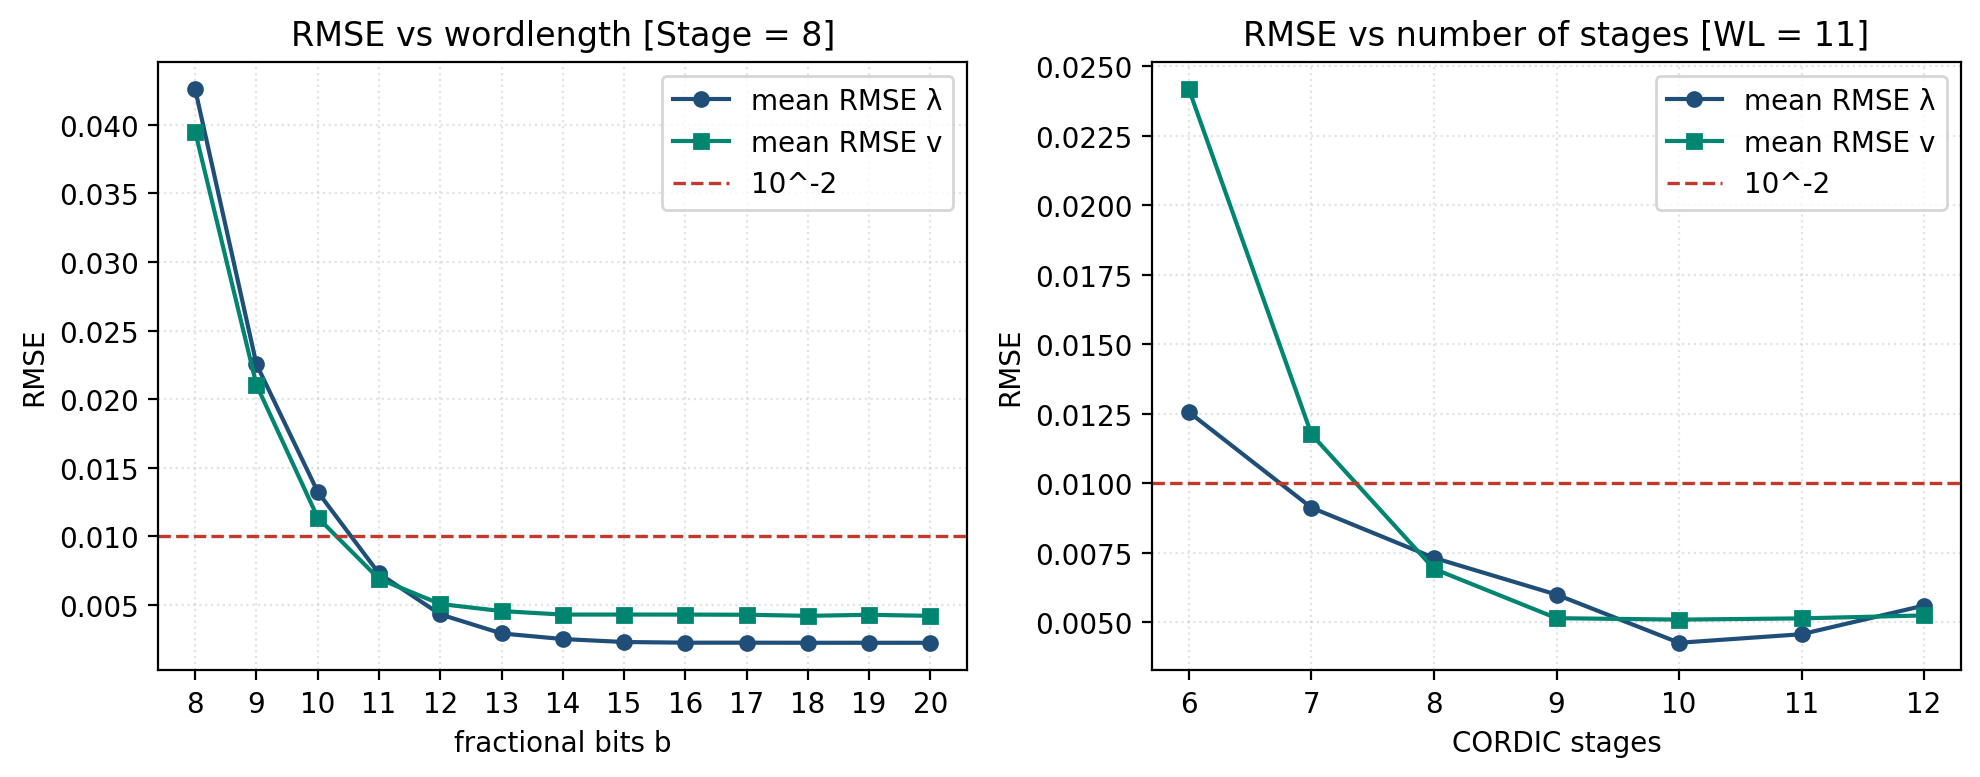
\includegraphics[width=\linewidth]{figure1.png}
    \caption{RMSE vs.\ fractional bits ($N_{\mathrm{stage}}=8$, left) and CORDIC stages ($b=11$, right).}
    \label{fig:rmse-1d}
\end{figure}

The two-step sweeps above are useful for intuition, but they do not jointly identify the smallest $(b, N_{\mathrm{stage}})$ pair.
Each pass fixes one parameter at the value found earlier, so a configuration that fails in isolation may still satisfy the RMSE criterion when both knobs are set together, and the true minimum combination may be missed.

\newpage

We therefore perform a two-dimensional sweep over fractional bits $b$ and CORDIC stages $N_{\mathrm{stage}}$.
Every grid point is evaluated on all 11 test patterns; a setting passes only when both $\mathrm{RMSE}_\lambda$ and $\mathrm{RMSE}_v$ remain below $10^{-2}$ for every set.

\begin{figure}[H]
    \centering
    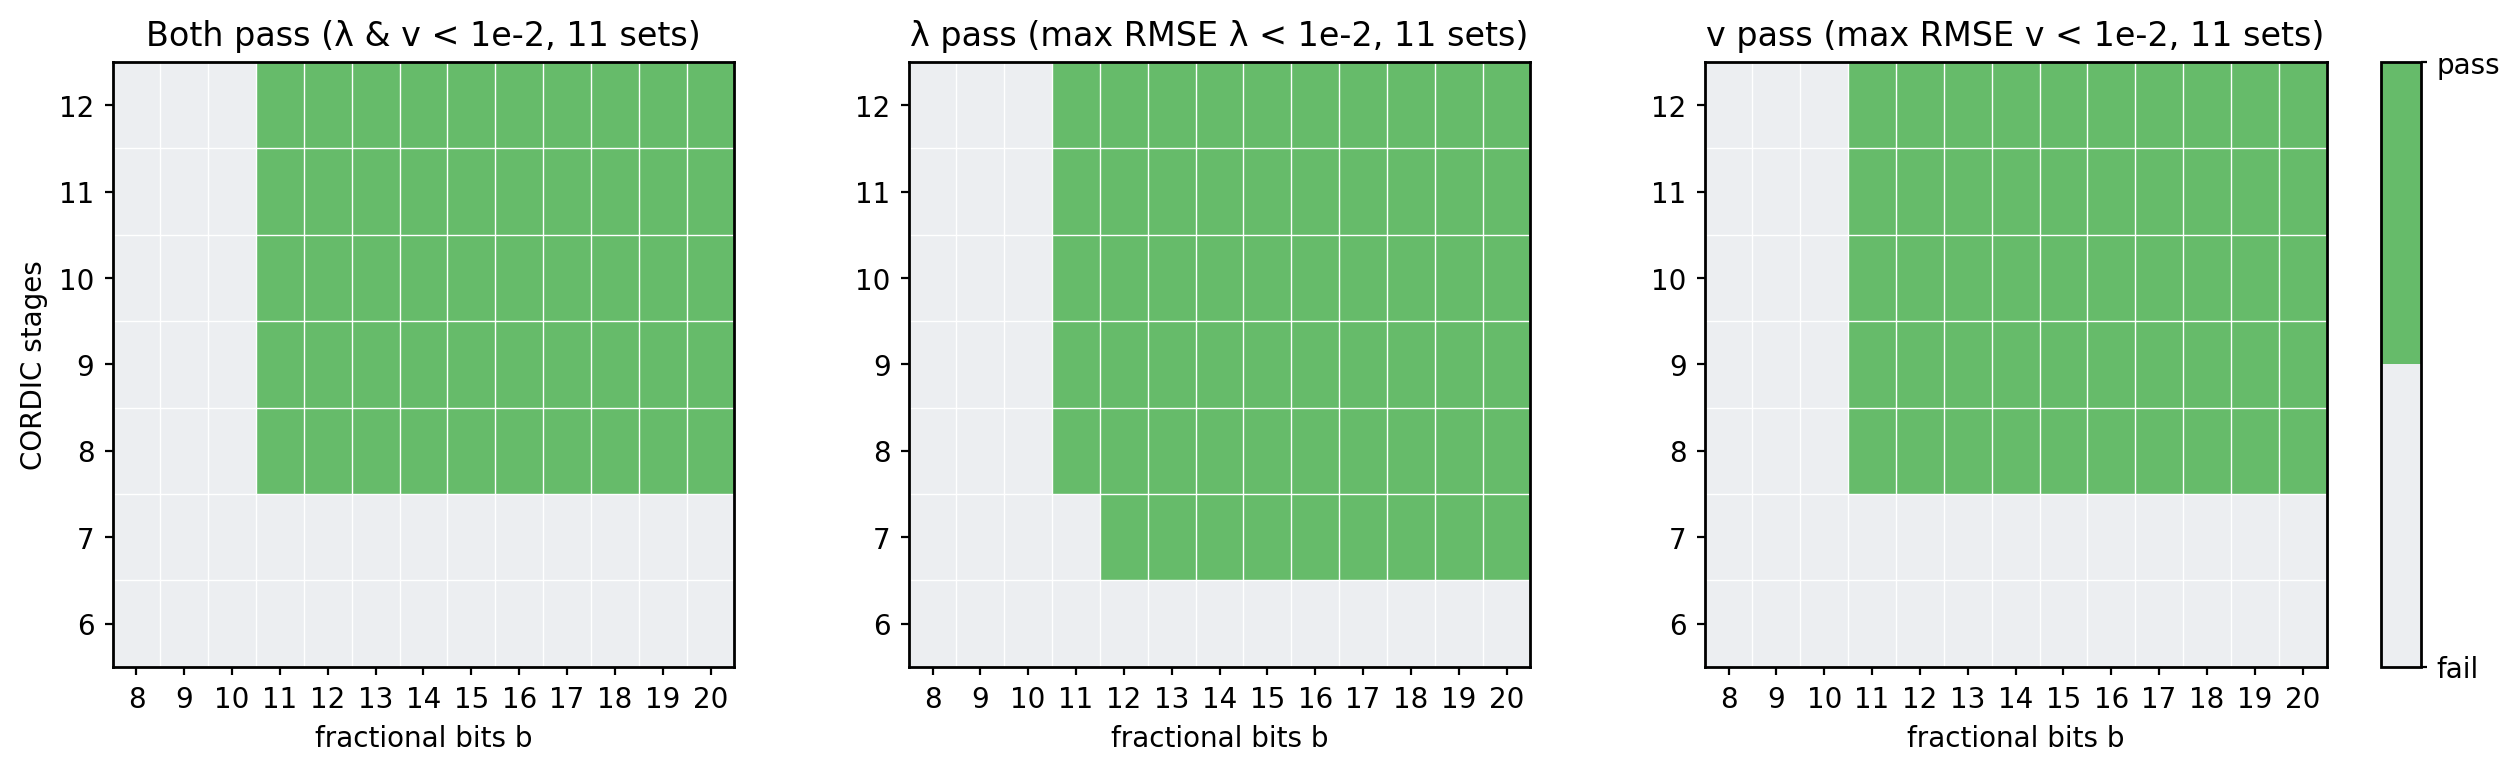
\includegraphics[width=\linewidth]{figure2.png}
    \caption{2D pass maps over $b$ and $N_{\mathrm{stage}}$ (11 test patterns).}
    \label{fig:rmse-2d}
\end{figure}

Table~\ref{tab:hw-config} summarizes the hardware configuration selected from the sweeps above.

\begin{table}[H]
\centering
\caption{Hardware Configuration}
\label{tab:hw-config}
\vspace{0.15em}
\setlength{\tabcolsep}{12pt}
\renewcommand{\arraystretch}{1.2}
\begin{tabular}{lc}
\toprule
\textbf{Parameter} & \textbf{Value} \\
\midrule
\texttt{B} (fractional bits)       & 11 \\
\texttt{N\_STAGES} (CORDIC stages) & 8 \\
\texttt{MAX\_ITER} (max iterations)  & 7 \\
\bottomrule
\end{tabular}
\end{table}

\section{Integer Bit-Width Analysis}

With the configuration in Table~\ref{tab:hw-config}, we record the dynamic range of each EVD stage across all 11 patterns and derive the minimum integer wordlength needed at each node.
Table~\ref{tab:int-bits} lists the worst-case integer bit requirement and the corresponding fixed-point format ($1$ sign bit + integer + $B$ fractional bits).

\begin{table}[H]
\centering
\caption{Integer Bit-Width Analysis}
\label{tab:int-bits}
\vspace{0.15em}
\setlength{\tabcolsep}{10pt}
\renewcommand{\arraystretch}{1.25}
\begin{tabular}{lrrrrlc}
\toprule
\textbf{Node} & \textbf{Min} & \textbf{Max} & \textbf{Max abs} & \textbf{Int.\ bits} & \textbf{Q format} & \textbf{Total} \\
\midrule
Quantized input   & $-2.394$ & $10.239$ & $10.239$ & 4 & Q4.11 & 16 \\
Matrix T/R        & $-5.117$ & $10.585$ & $10.585$ & 4 & Q4.11 & 16 \\
Eigenvector U     & $-0.981$ & $1.000$  & $1.000$  & 1 & Q1.11 & 13 \\
CORDIC input      & $-5.117$ & $10.585$ & $10.585$ & 4 & Q4.11 & 16 \\
CORDIC internal   & $-10.586$ & $17.432$ & $17.432$ & 5 & Q5.11 & 17 \\
Scaled output     & $-5.117$ & $10.585$ & $10.585$ & 4 & Q4.11 & 16 \\
\bottomrule
\end{tabular}
\end{table}

\newpage

\section{Fixed-Point Bit-True Model}

With the fractional wordlength, CORDIC stage count, iteration limit, and integer bit-width requirements established above, we implement a fixed-point bit-true model of the iterative QR EVD datapath.
The model applies the formats in Tables~\ref{tab:hw-config} and~\ref{tab:int-bits} at each quantization point so that its arithmetic matches the behavior targeted by the RTL design.

This model supports more accurate fixed-point error analysis than a floating-point reference, because quantization, CORDIC rounding, and iterative accumulation are modeled explicitly.
It also supplies golden eigenvalues and eigenvectors for RTL verification, so behavior and gate-level simulations can be compared against a consistent fixed-point reference instead of double-precision software alone.

\section{CORDIC Scaling Factor}

Sections~\ref{fig:rmse-1d}--\ref{tab:int-bits} do not analyze the impact of quantizing the CORDIC scaling factor.
They model gain compensation as $Q_B(X/K)$ only (divide by ideal $K$), then quantize the quotient.
This is intentional, we do not want scaling-factor precision to enlarge global fractional bits $B$ and widen the entire systolic datapath.
Therefore, Extra bits are spent only at this multiply-and-round point, not across the systolic array.

\begin{table}[H]
\centering
\caption{CORDIC Scaling Factor Configuration}
\label{tab:k-config}
\vspace{0.15em}
\setlength{\tabcolsep}{12pt}
\renewcommand{\arraystretch}{1.2}
\begin{tabular}{lc}
\toprule
\textbf{Parameter} & \textbf{Value} \\
\midrule
\texttt{DATA\_FRAC} (datapath fractional bits)     & 11 \\
\texttt{DATA\_WIDTH} (datapath total bits) & 17 \\
\texttt{K\_INV\_FRAC} (fractional bits for $1/K$) & 16 \\
\texttt{K\_INV\_DW} (total bits for $1/K$) & 17 \\
\bottomrule
\end{tabular}
\end{table}

\section{CSD vs Constant Multiplier}

For CORDIC gain compensation ($X \times (1/K)$), we compared a hand-designed CSD multiplier with a constant multiplier left for Design Compiler to optimize.
In our synthesis experiments, the CSD path introduces truncation error.
A custom CSD design that meets the same accuracy requirement is larger than the constant multiplier optimized by Design Compiler.
We therefore use the Design Compiler-optimized constant multiplier in the final RTL.

% ─────────────────────────────────────────────
\chapter{Section 2: Bit-True Model Verification}
% ─────────────────────────────────────────────

\section{RMSE Per Pattern}

We evaluate the bit-true model on all 11 patterns in \texttt{Final11Pattern.mat} with $B = 11$, $N_{\mathrm{stage}} = 8$, and $\mathrm{MAX\_ITER} = 7$.
Figure~\ref{fig:rmse-patterns} plots $\mathrm{RMSE}_\lambda$ and $\mathrm{RMSE}_v$ per pattern; both remain below $10^{-2}$.

\begin{figure}[H]
    \centering
    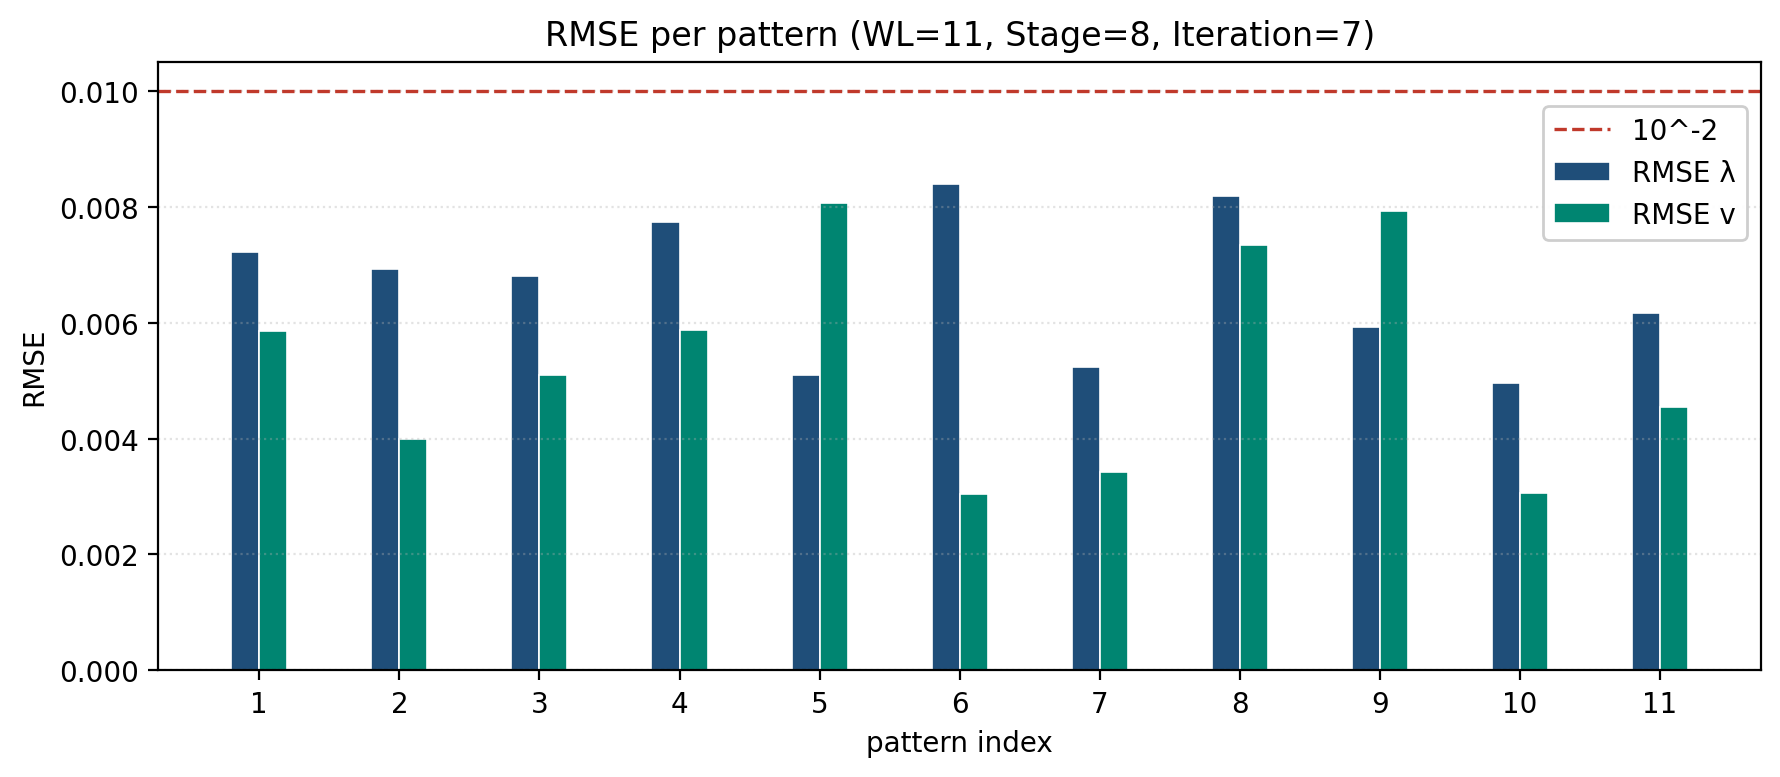
\includegraphics[width=\linewidth]{figure3.png}
    \caption{RMSE per pattern.}
    \label{fig:rmse-patterns}
\end{figure}

\newpage

% ─────────────────────────────────────────────
\chapter{Section 3: Hardware Architecture and Control}
% ─────────────────────────────────────────────

\section{CORDIC PE Architecture}

We follow the \href{https://github.com/akira2963753/DSP-In-VLSI/tree/master/HW4-CORDIC/Final}{Homework~4} CORDIC PE design: inputs are preconditioned in the initial stage, and the eight CORDIC micro-rotation stages are unfolded and pipelined to maximize throughput.
For this EVD application, \textbf{the exact rotation angle $\theta$ does not need to be stored.}
Vectoring mode records each micro-rotation direction in a rotational direction register (RDR) and rotation mode replays those directions on the remaining matrix entries.

All $\theta$-related arithmetic in the CORDIC datapath can therefore be removed, improving PPA (power, performance, and area).
Figure~\ref{fig:cordic-pe} shows the resulting PE architecture.

\begin{figure}[H]
    \centering
    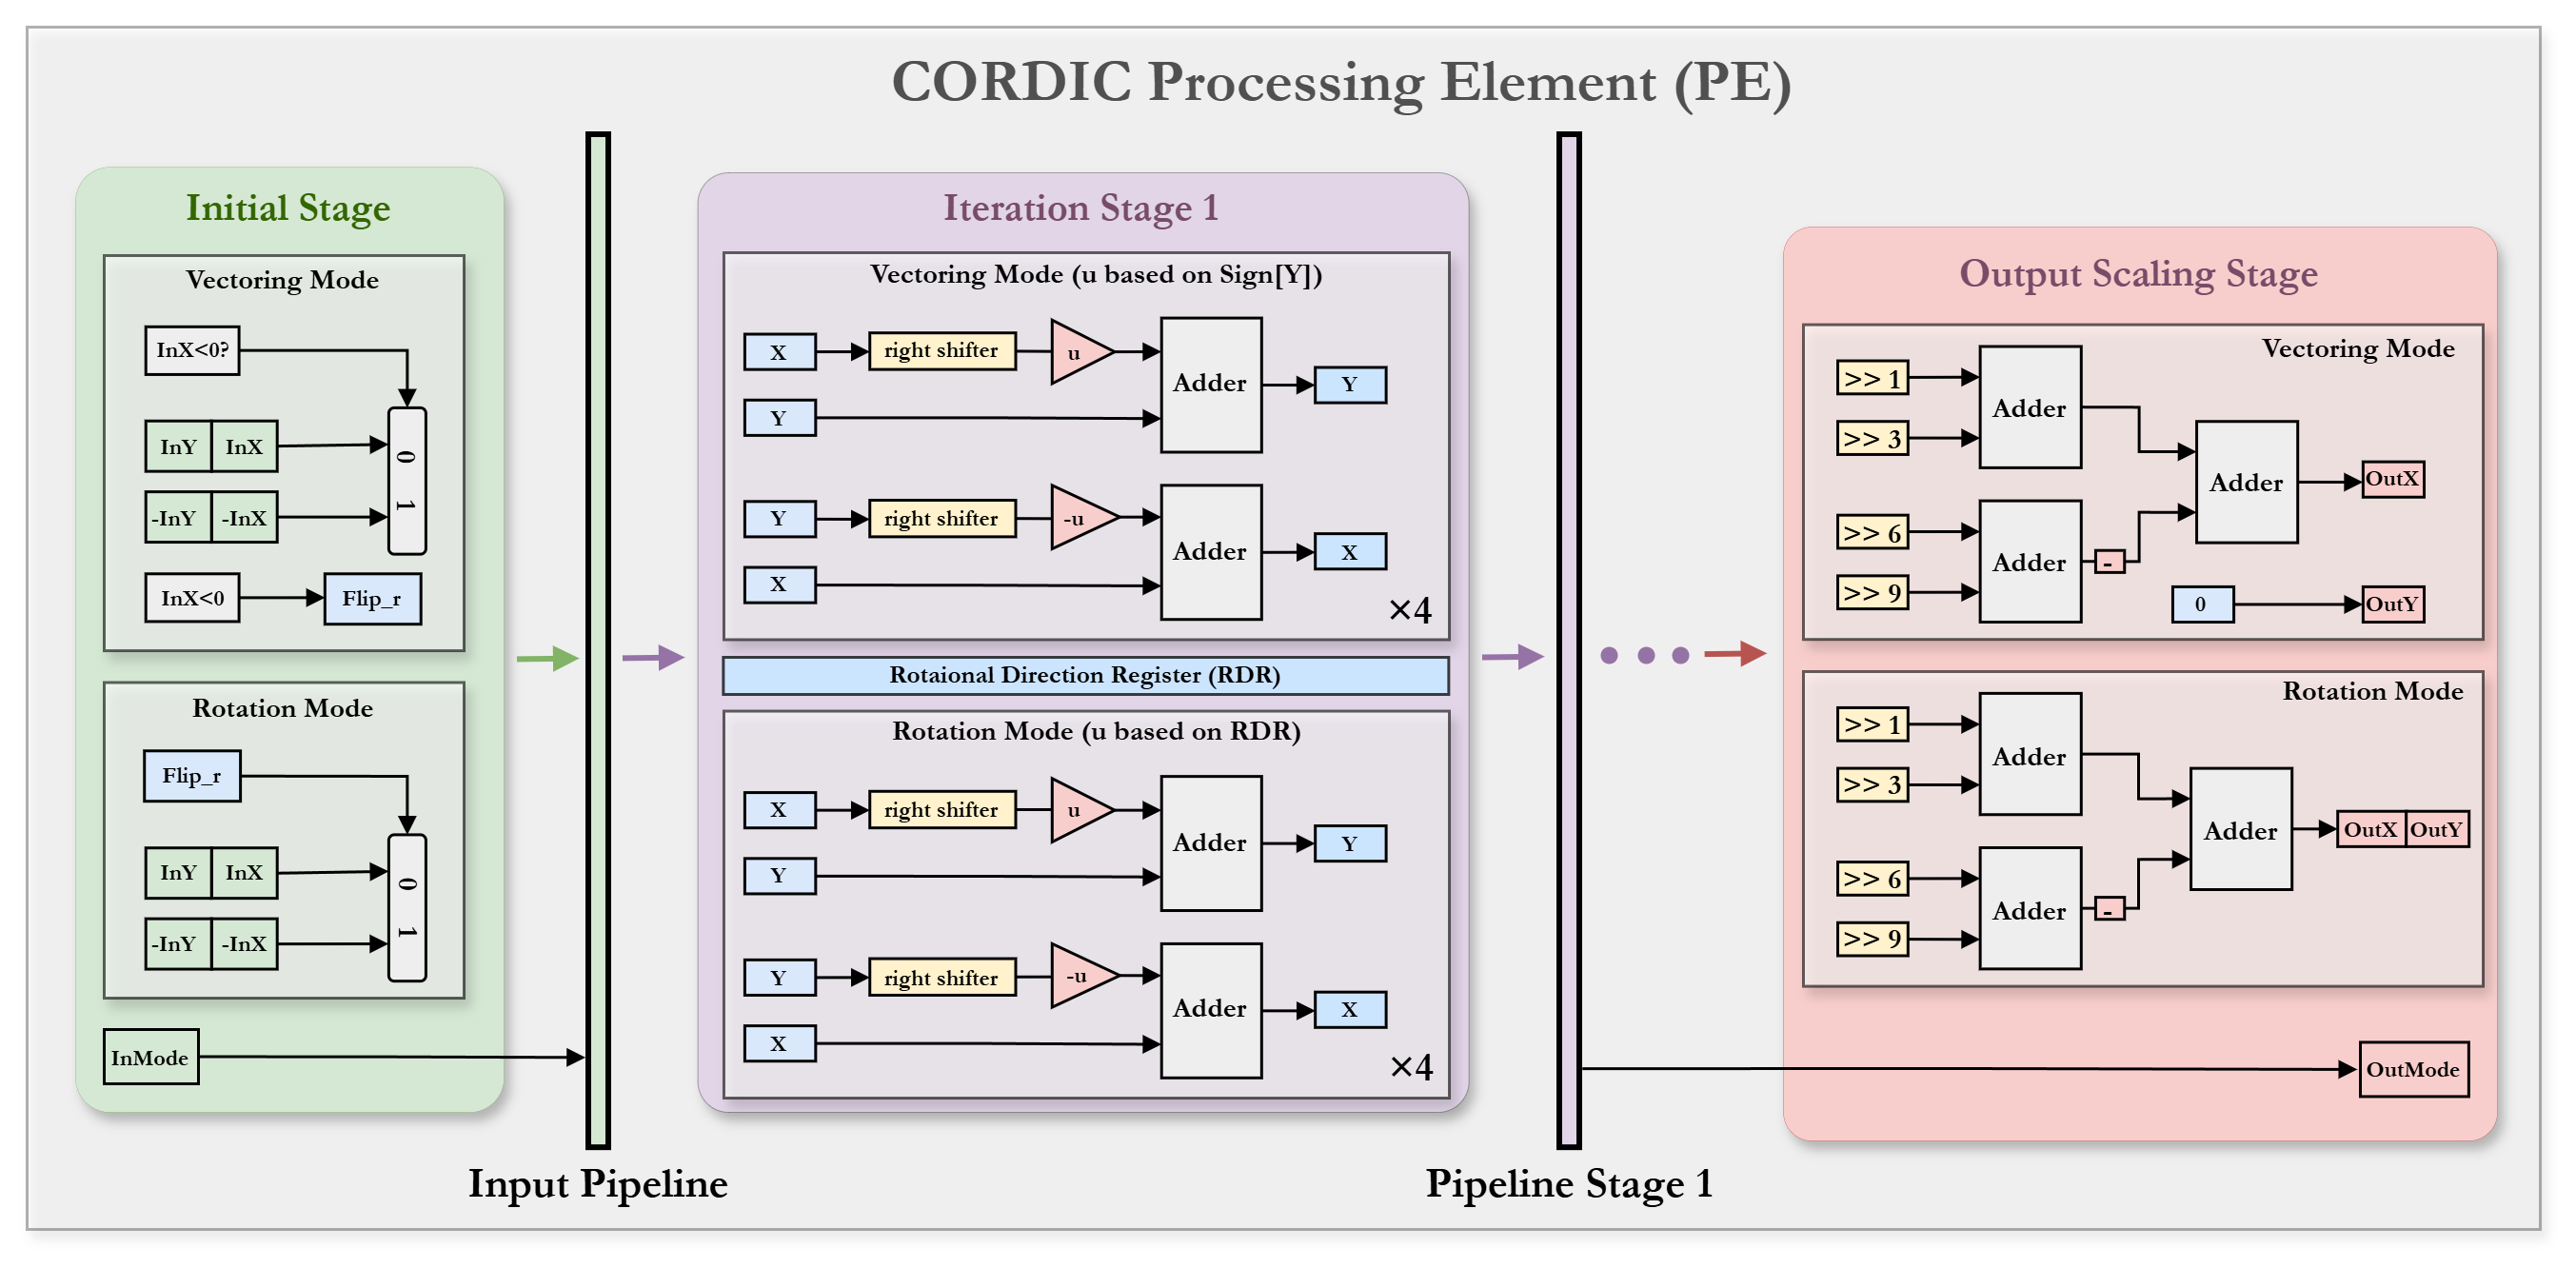
\includegraphics[width=\linewidth]{CORDIC_PE.png}
    \caption{CORDIC PE Architecture.}
    \label{fig:cordic-pe}
\end{figure}

Figure~\ref{fig:cordic-pe} shows that the second iteration stage feeds directly into the output scaling stage.
For better PPA, the two pipeline stages need not perform the same number of micro-rotations.
The first iteration stage can execute five micro-rotations and the second stage three, while still completing all eight stages before gain compensation.

\newpage

\section{Systolic Array-Based QRD Architecture}

Each CORDIC PE produces one result every two cycles, so the triangular QRD systolic array is retimed around this two-cycle latency.
\textbf{We remove the delay unit at the bottom-right diagonal position} to keep the array outputs aligned.
The detailed timing schedule is given in the next section.

Figure~\ref{fig:qrd-systolic} shows the resulting array: 
three CORDIC PE blocks (2-cycle), one single-cycle Delay Unit, and one two-cycle Delay 2 Unit.

\begin{figure}[H]
    \centering
    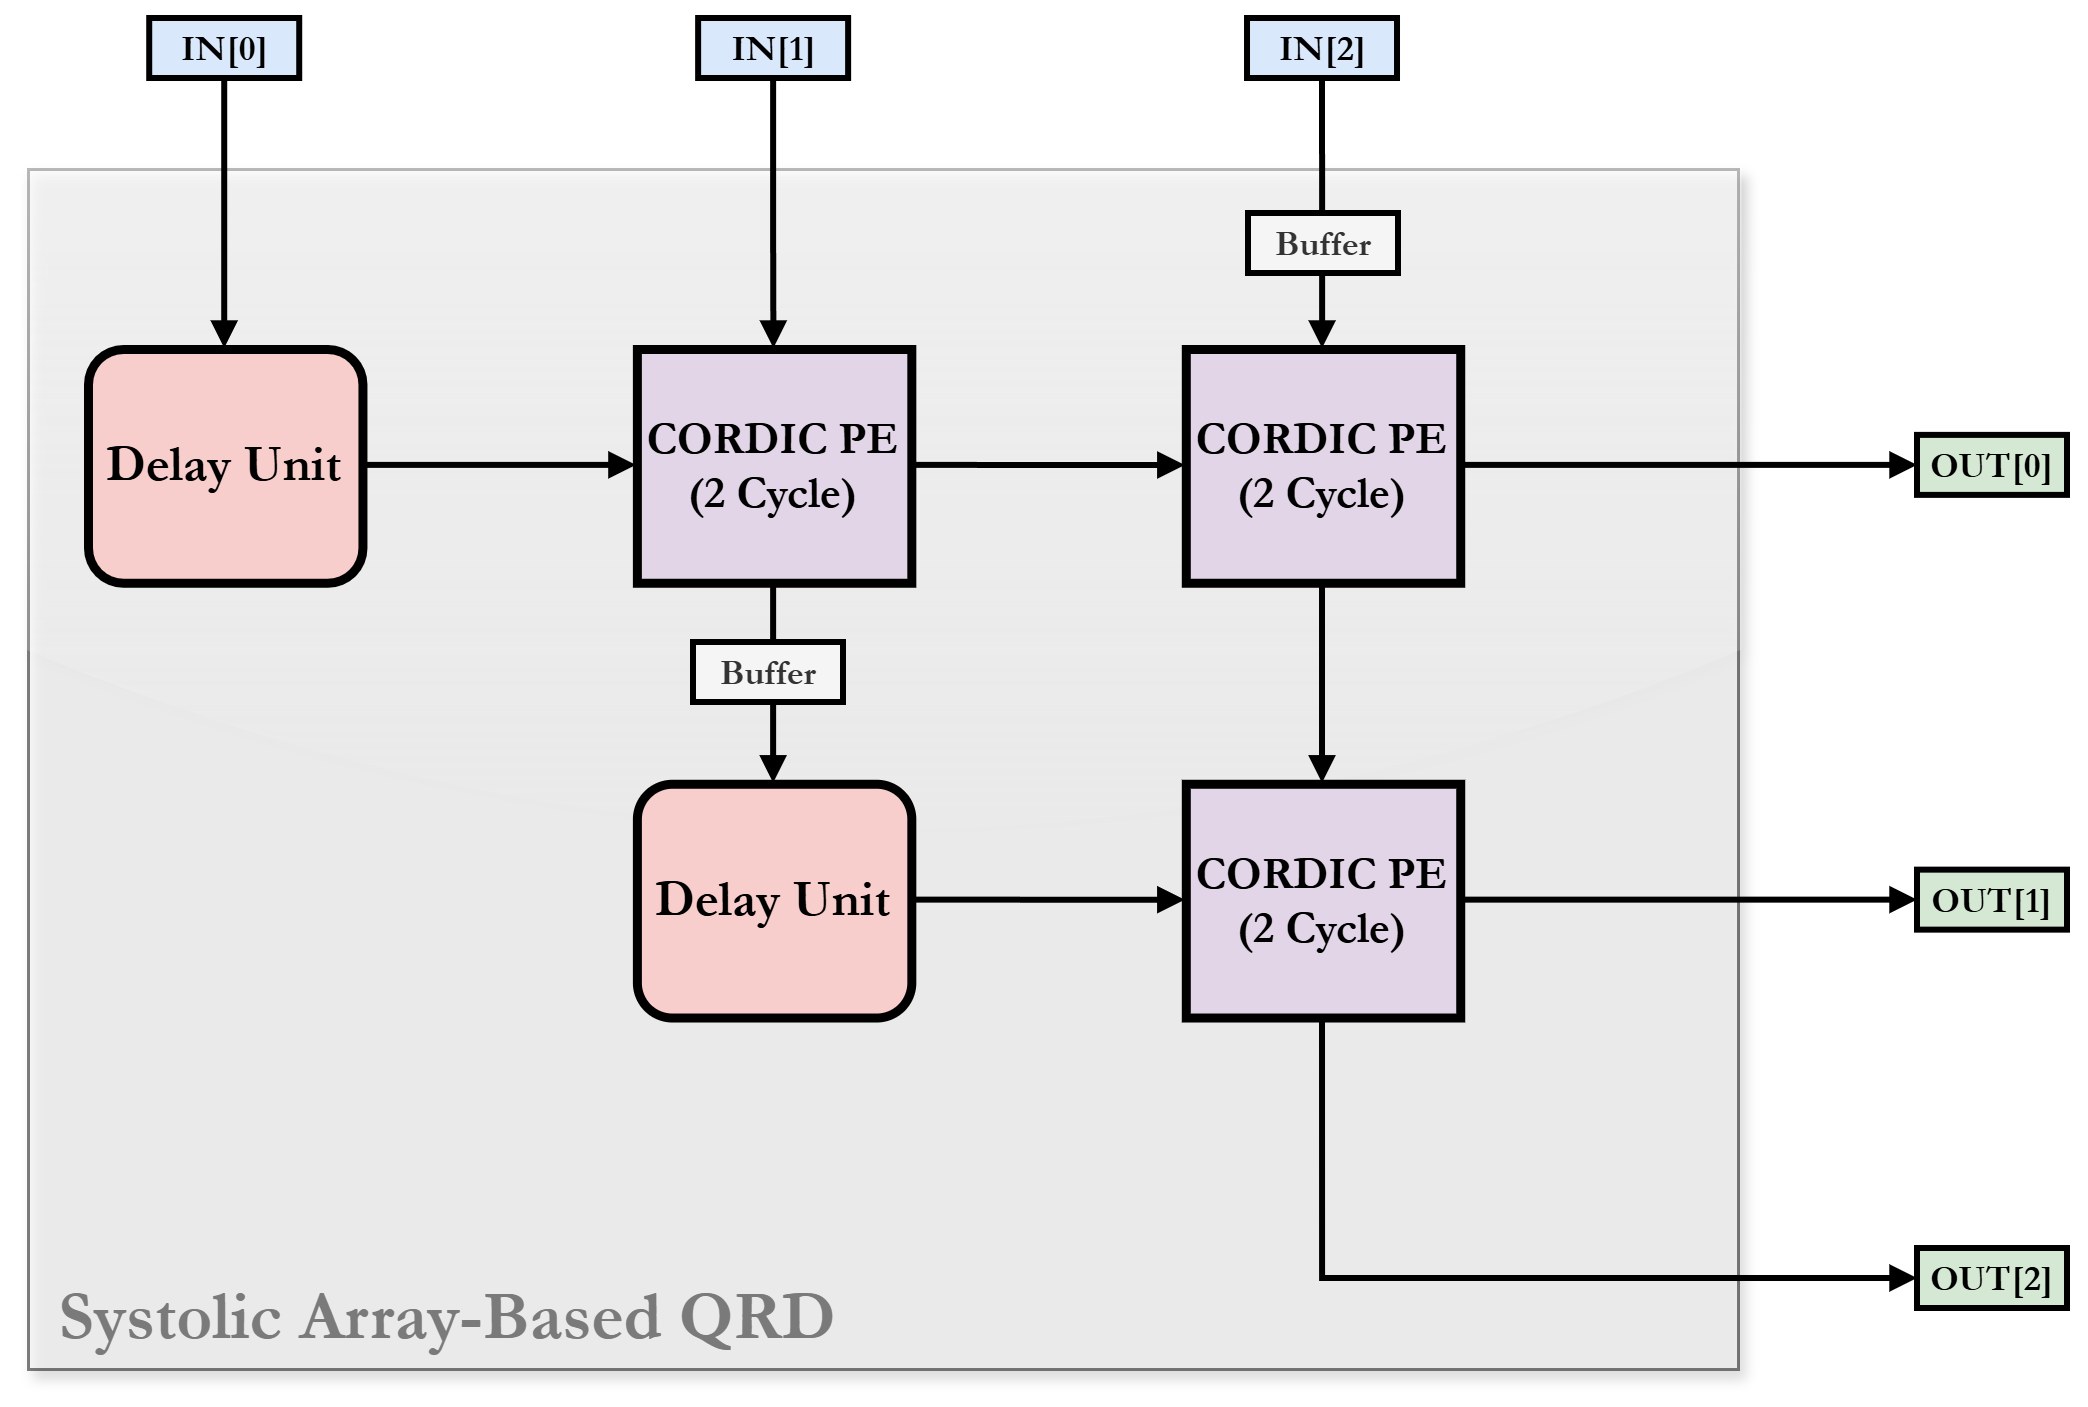
\includegraphics[width=0.85\linewidth]{QRD-Systolic-Array.png}
    \caption{Systolic array-based QRD architecture.}
    \label{fig:qrd-systolic}
\end{figure}

\newpage

\section{EVD Architecture}

The top-level EVD module wraps the QRD systolic array with an input delay unit (IDU), matrix registers, and a three-state FSM.
Table~\ref{tab:evd-fsm} summarizes the control flow. Figure~\ref{fig:evd-timing} gives the cycle-by-cycle hardware schedule.

\begin{table}[H]
\centering
\caption{EVD FSM States}
\label{tab:evd-fsm}
\vspace{0.15em}
\setlength{\tabcolsep}{10pt}
\renewcommand{\arraystretch}{1.2}
\begin{tabularx}{\textwidth}{>{\centering\arraybackslash}p{1.5cm} >{\centering\arraybackslash}X}
\toprule
\textbf{State} & \textbf{Function} \\
\midrule
\texttt{IDLE} &
When InValid is asserted, stream the external $3 \times 3$ input matrix into the systolic array over three cycles, then enter \texttt{PROCESS}. \\
\texttt{PROCESS} &
Run seven QR iterations.
Each iteration takes 15 cycles: feed $U$ for eigenvector update, feed $R^{\mathsf{T}}$ for $T$ update, then feed the updated $T$ back into the array. \\
\texttt{OUT} &
After the seventh iteration, stream the eigenvalues and the three rows of $U$ (eigenvectors) to the output ports over four cycles, then return to \texttt{IDLE}. \\
\bottomrule
\end{tabularx}
\end{table}

In \texttt{PROCESS}, the FSM counter (cnt) schedules reads from the U Register, updates to the Output Buffer, and systolic handshaking so that inputs and outputs remain aligned with the two-cycle CORDIC PE latency.
Figure~\ref{fig:evd-timing} tabulates this schedule for the \texttt{IDLE} load phase and one \texttt{PROCESS} iteration.

It is worth noting that lifetime-table analysis of the Output Buffer shows that the minimum number of registers required is \textbf{five}.

\begin{figure}[H]
    \centering
    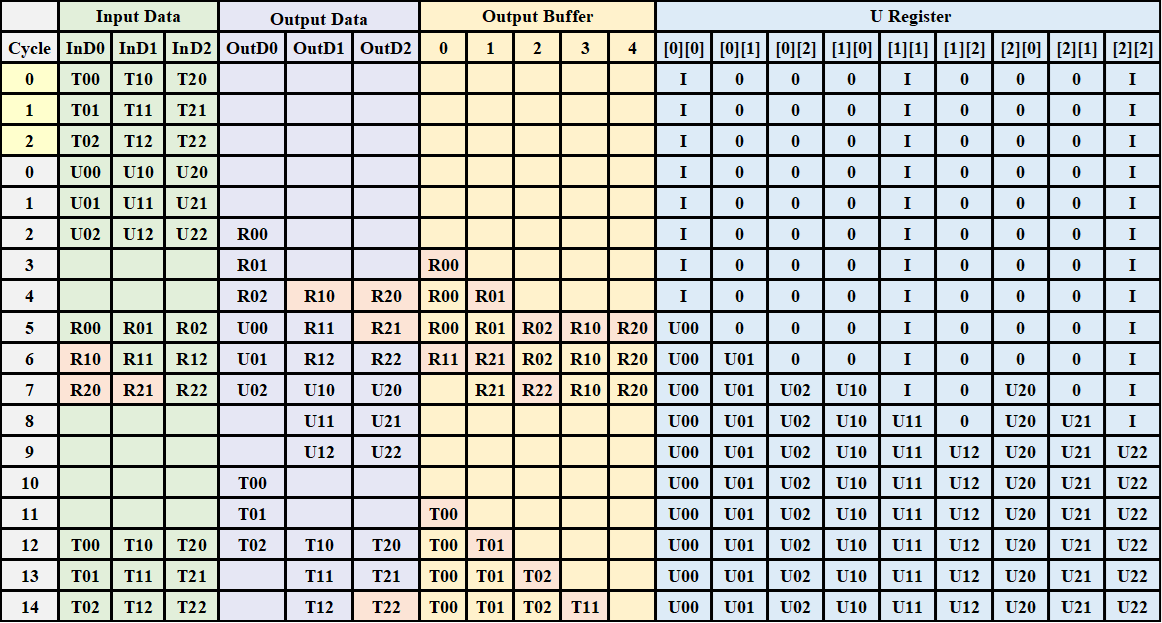
\includegraphics[width=\linewidth]{figure4.png}
    \caption{Hardware timing schedule (\texttt{IDLE} input load and one \texttt{PROCESS} iteration).}
    \label{fig:evd-timing}
\end{figure}

\newpage

According the Figure~\ref{fig:evd-timing}, One complete EVD run finishes in \textbf{112 clock cycles} from input load to the last output word.
Table~\ref{tab:evd-latency} breaks this down by FSM phase.

\begin{table}[H]
\centering
\caption{EVD Latency}
\label{tab:evd-latency}
\vspace{0.15em}
\setlength{\tabcolsep}{12pt}
\renewcommand{\arraystretch}{1.2}
\begin{tabular}{lc}
\toprule
\textbf{Phase} & \textbf{Cycles} \\
\midrule
\texttt{IDLE} (input load)                    & 3 \\
\texttt{PROCESS} ($7$ iterations $\times$ $15$ cycles) & 105 \\
\texttt{OUT} (eigenvalues and eigenvectors)   & 4 \\
\midrule
\textbf{Total}                                & \textbf{112} \\
\bottomrule
\end{tabular}
\end{table}

A three-state FSM controls the datapath according to the schedule in Figure~\ref{fig:evd-timing}.
The pre-processor selects the systolic-array inputs on each cycle (external matrix, U Register, or Output Buffer), and the IDU aligns them with the two-cycle CORDIC PE latency.
$R$ and $T$ are staged in an Output Buffer. $U$ is stored in a U Register.
In \texttt{PROCESS}, the FSM reads both buffers and feeds the array for each QR iteration.
In \texttt{OUT}, eigenvalues come from the Output Buffer and eigenvectors from the U Register.
Figure~\ref{fig:evd-arch} shows the top-level architecture.

\begin{figure}[H]
    \centering
    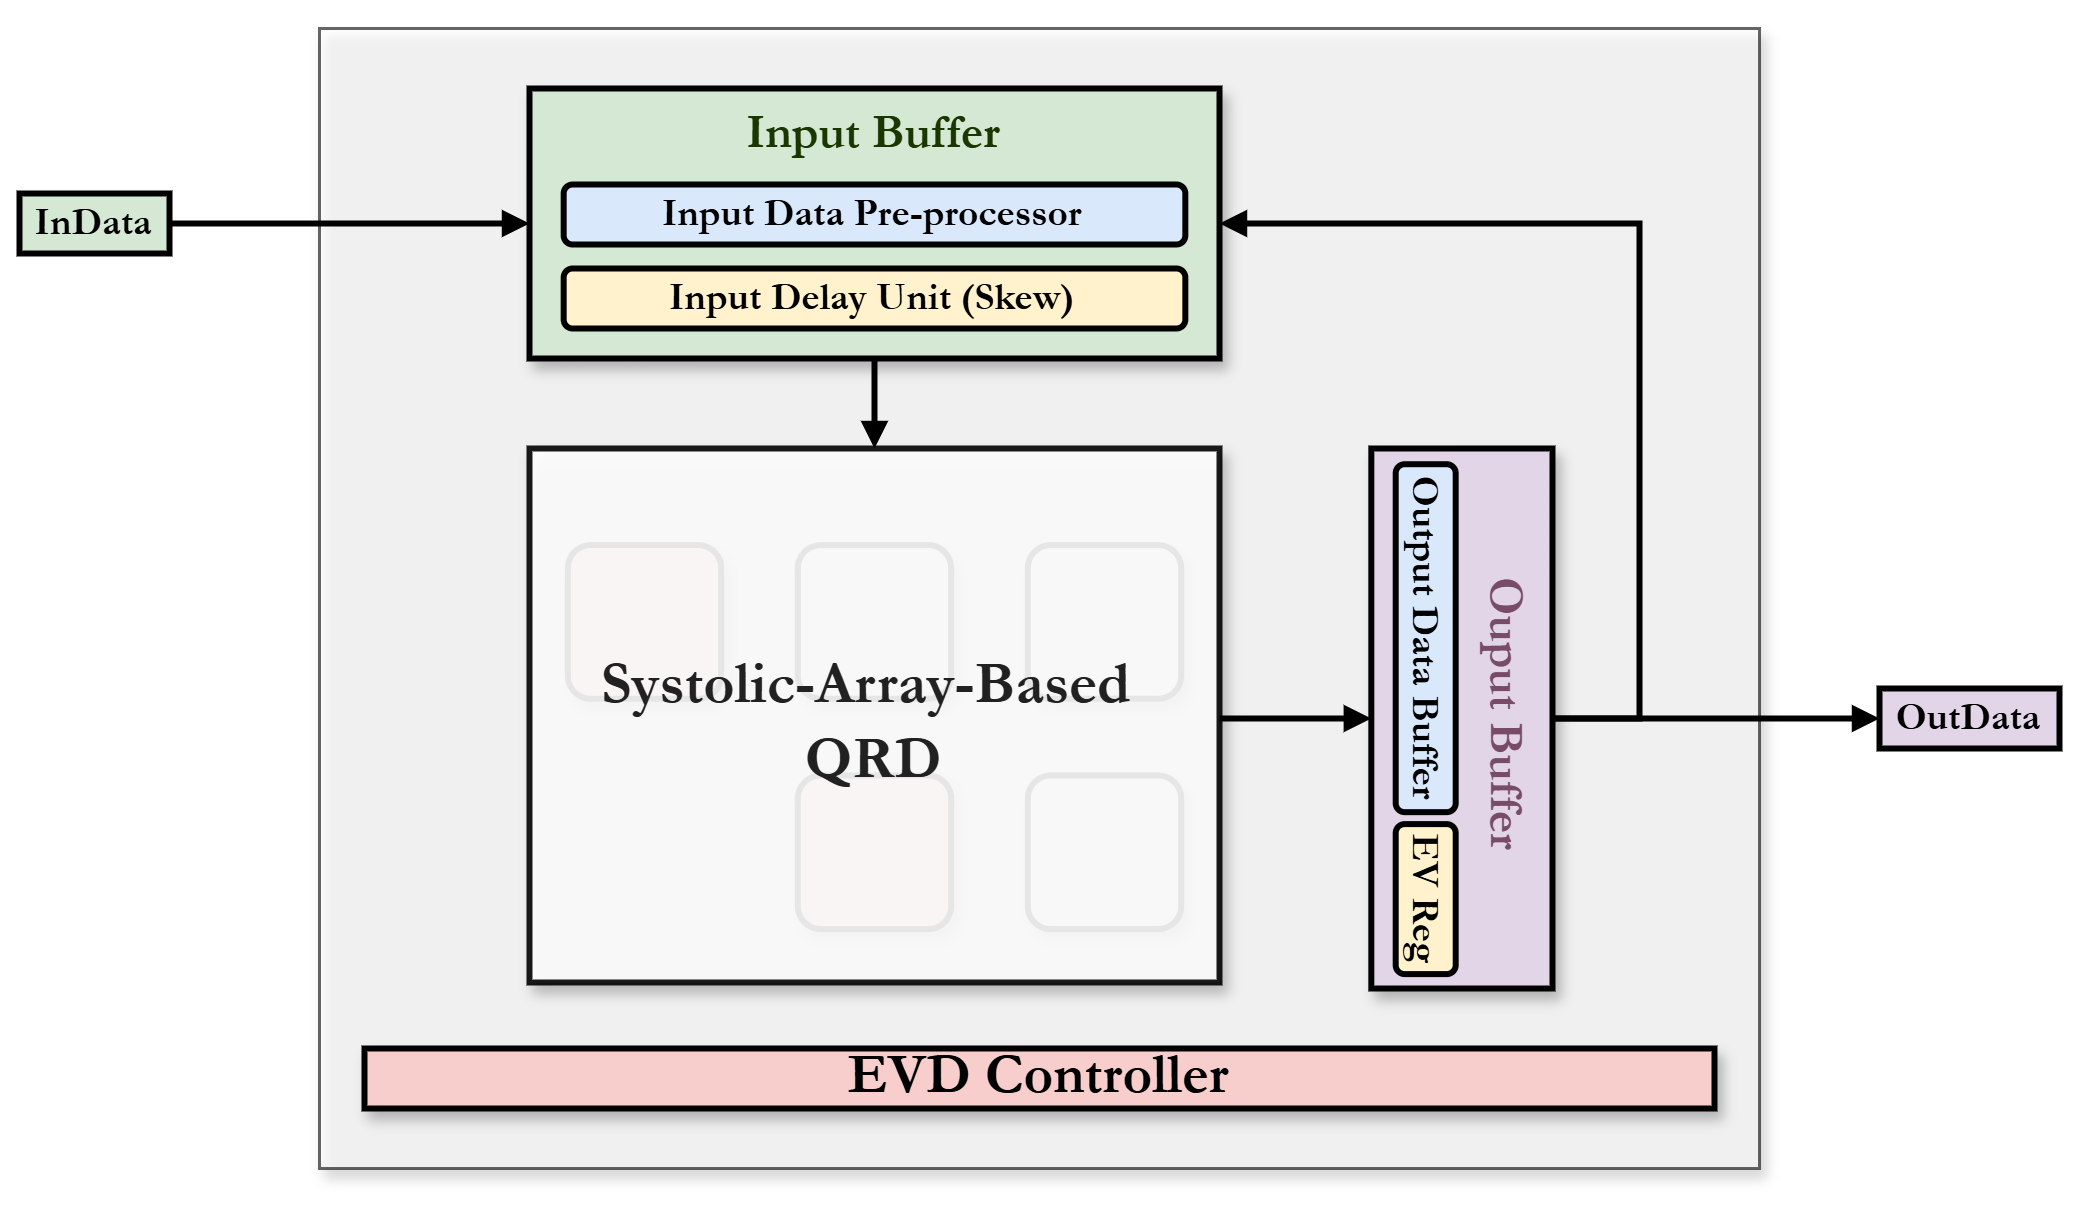
\includegraphics[width=\linewidth]{EVD.png}
    \caption{Top-level EVD architecture.}
    \label{fig:evd-arch}
\end{figure}

\newpage

\section{Detailed Transpose Buffer (Output Buffer)}

The Output Buffer is the transpose buffer that feeds $\mathbf{R}^{\mathsf{T}}$ back
into the array to form $\mathbf{R}\mathbf{Q}$. It is simply the direct hardware
realization of the timing schedule of Fig.~\ref{fig:evd-timing}: the whole iterative
operation is sequenced by a single FSM counter \texttt{cnt}, which on each cycle
selects both the register written from the array output and the registers read back
into the array. No separate addressing logic is needed; \texttt{cnt} alone drives the
write and the transposed read-back.

Figure~\ref{fig:transpose-buffer} shows the buffer at cnt~$=5$, $6$, and $7$; the
circled \texttt{cnt} value marks when each register was written, and the five
registers are read in transposed order to form the three input rows of
$\mathbf{R}^{\mathsf{T}}$.

\begin{figure}[H]
    \centering
    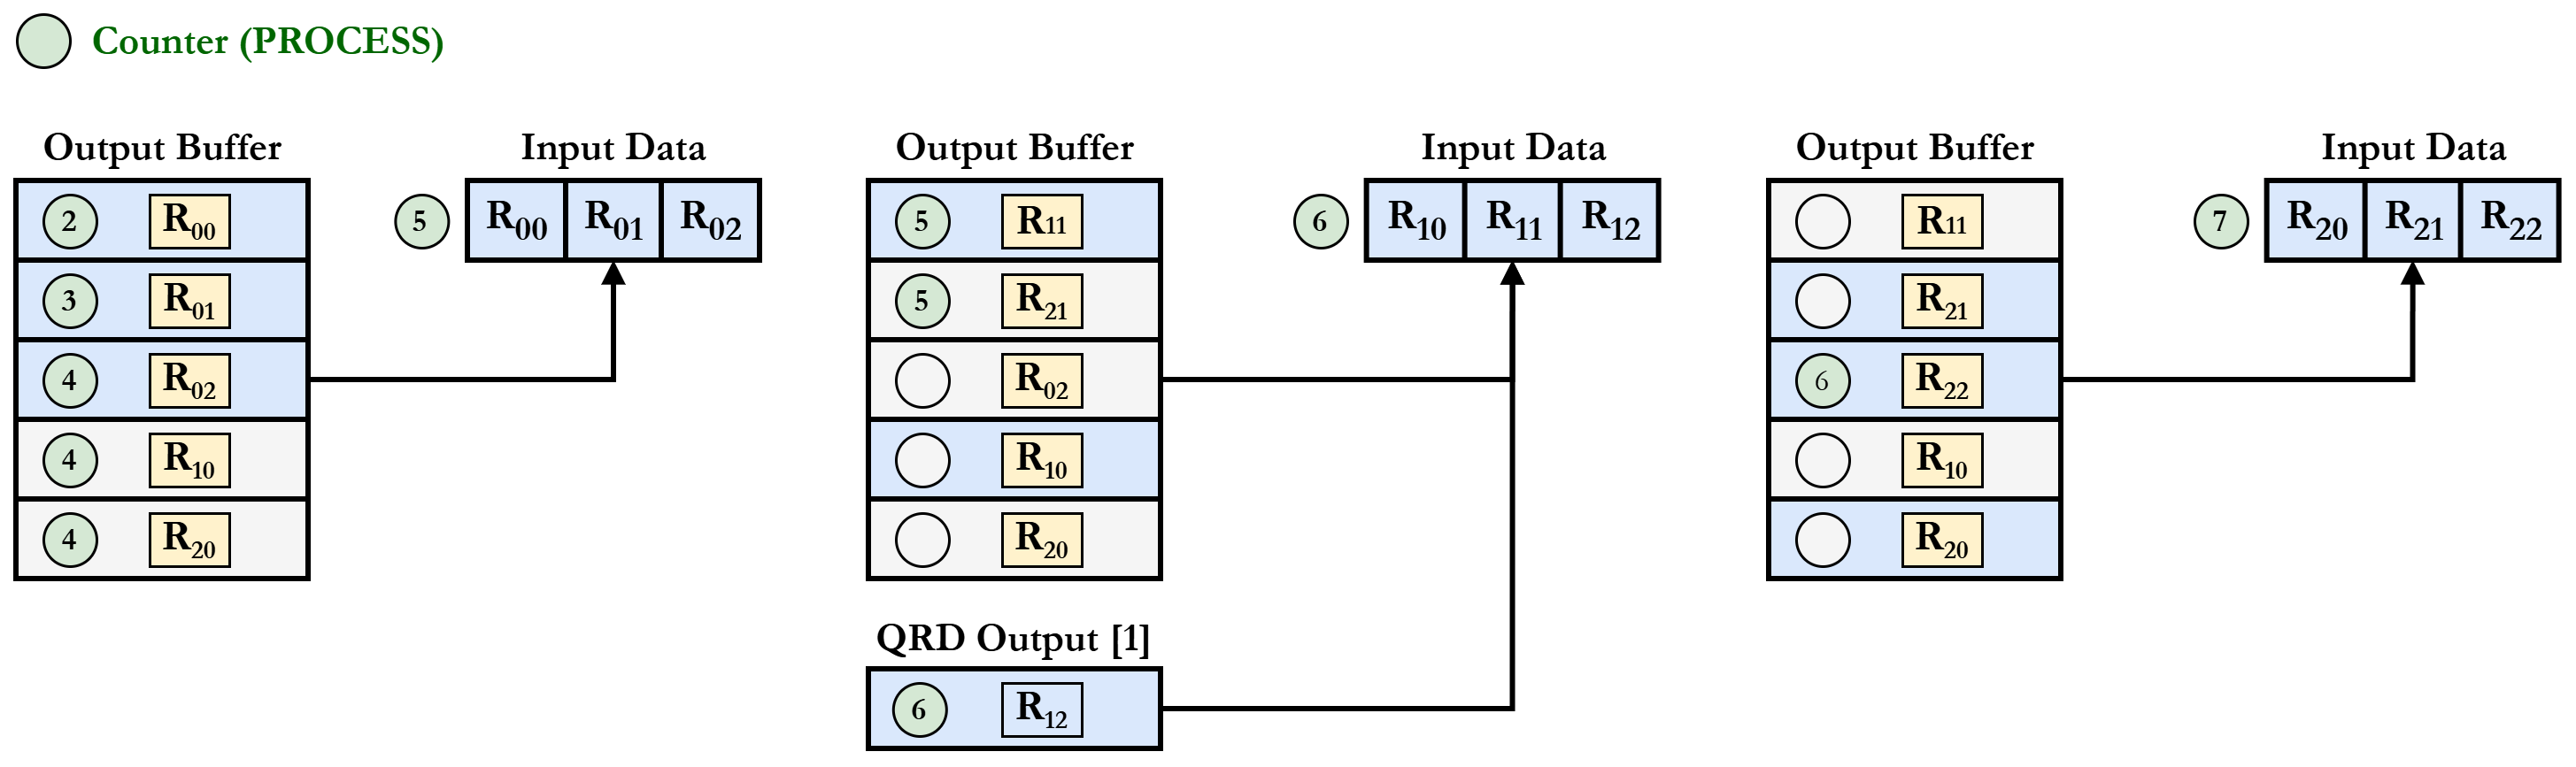
\includegraphics[width=\linewidth]{OutputBuffer.png}
    \caption{Transpose buffer (Output Buffer) Block Diagram.}
    \label{fig:transpose-buffer}
\end{figure}


% ─────────────────────────────────────────────
\chapter{Section 4: Hardware Simulation}
% ─────────────────────────────────────────────

\section{Behavioral Simulation}
We verify the RTL with Synopsys VCS and inspect waveforms in Verdi.
Figure~\ref{fig:hw-sim-input} shows the \texttt{IDLE} phase: \texttt{InValid} is held
for three cycles while the input matrix is streamed column-by-column on
\texttt{InData}.
Figure~\ref{fig:hw-sim-output} shows the \texttt{OUT} phase: after processing completes,
\texttt{OutValid} is asserted for four cycles while the eigenvalues and the three rows
of $U$ appear on \texttt{OutData}.

\begin{figure}[H]
    \centering
    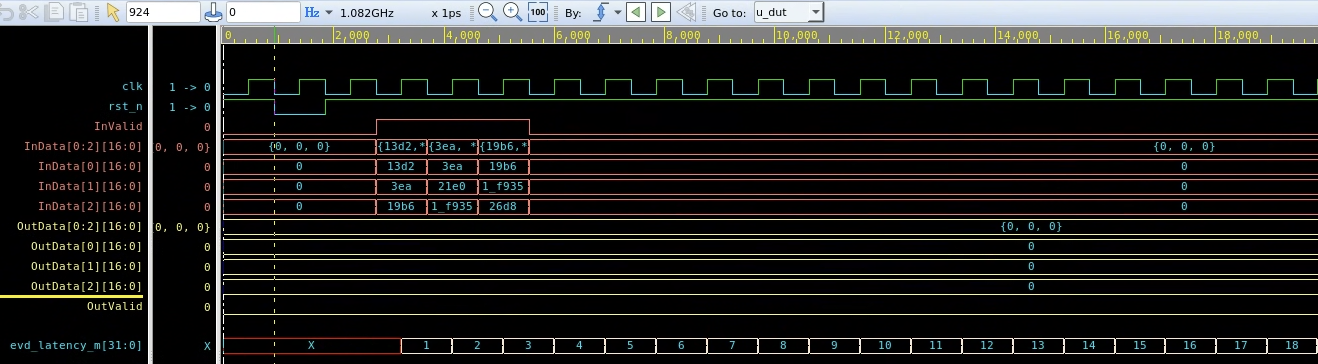
\includegraphics[width=\linewidth]{Waveform1.png}
    \caption{RTL simulation waveform: input matrix load (\texttt{IDLE}).}
    \label{fig:hw-sim-input}
\end{figure}

\begin{figure}[H]
    \centering
    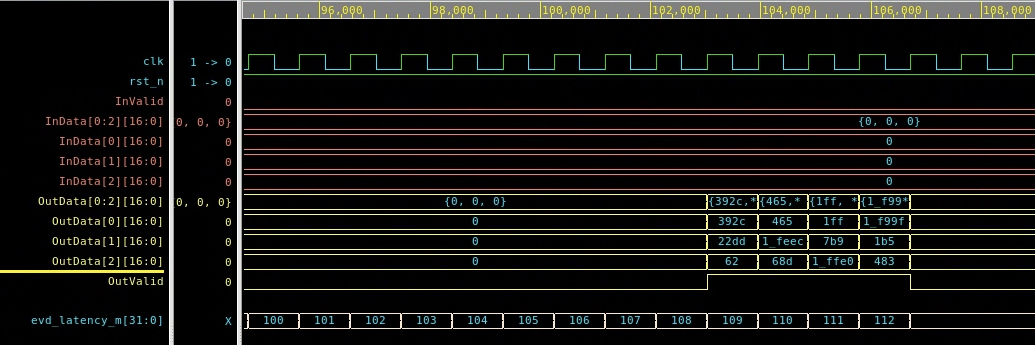
\includegraphics[width=\linewidth]{Waveform2.png}
    \caption{RTL simulation waveform: eigenvalue/eigenvector output (\texttt{OUT}).}
    \label{fig:hw-sim-output}
\end{figure}

The testbench exposes a latency monitor \texttt{evd\_latency\_m} that increments on every
clock cycle from the rising edge of \texttt{InValid} until the falling edge of
\texttt{OutValid}.
As shown in the waveforms, one complete EVD run finishes in \textbf{112 clock cycles},
consistent with the latency breakdown in Table~\ref{tab:evd-latency}.

\newpage

\section{Post-Synthesis Simulation}

We run gate-level simulation at the best-ATP from section 6, whose clock period
is \textbf{923,437 fs} (see the time scale in the upper-right corner of
Figures~\ref{fig:post-syn-input} and~\ref{fig:post-syn-output}).
The waveforms show that the results are fully consistent with the behavioral
simulation.

\begin{figure}[H]
    \centering
    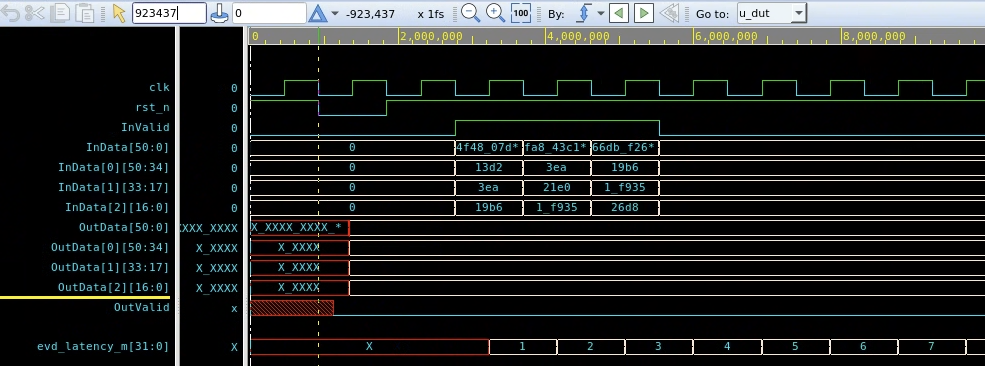
\includegraphics[width=\linewidth]{Waveform3.png}
    \caption{Post-synthesis simulation waveform.}
    \label{fig:post-syn-input}
\end{figure}

\begin{figure}[H]
    \centering
    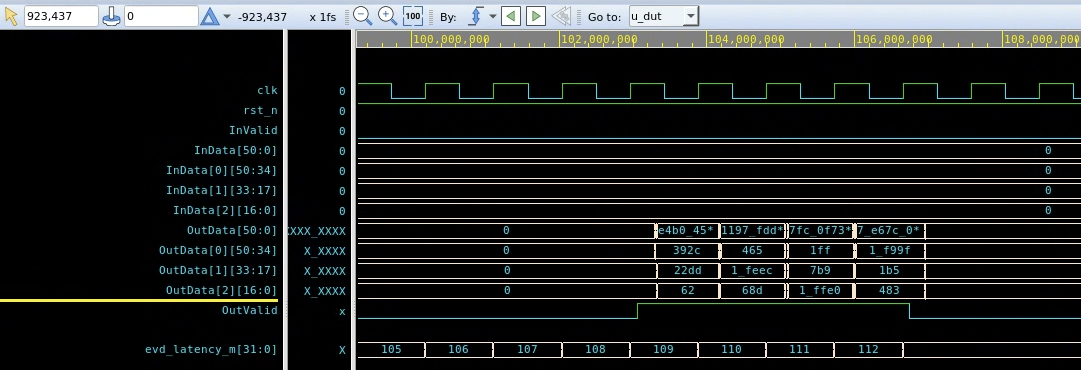
\includegraphics[width=\linewidth]{Waveform4.png}
    \caption{Post-synthesis simulation waveform.}
    \label{fig:post-syn-output}
\end{figure}

For the required \textbf{test pattern 8}, the behavioral simulation yields
$\mathrm{RMSE}_\lambda = 5.923380 \times 10^{-3}$ and
$\mathrm{RMSE}_v = 7.921108 \times 10^{-3}$, both below the $10^{-2}$ criterion.

\newpage

\section{Fixed-Point vs.\ Hardware Consistency}

Hardware outputs match the fixed-point bit-true model exactly on every test pattern.

Figure~\ref{fig:rmse-patterns} plots the per-pattern RMSE against the reference;
both $\mathrm{RMSE}_\lambda$ and $\mathrm{RMSE}_v$ remain below $10^{-2}$ for all
11 patterns.
Figure~\ref{fig:hw-consistency} shows pattern~8 as an example.

\begin{figure}[H]
    \centering
    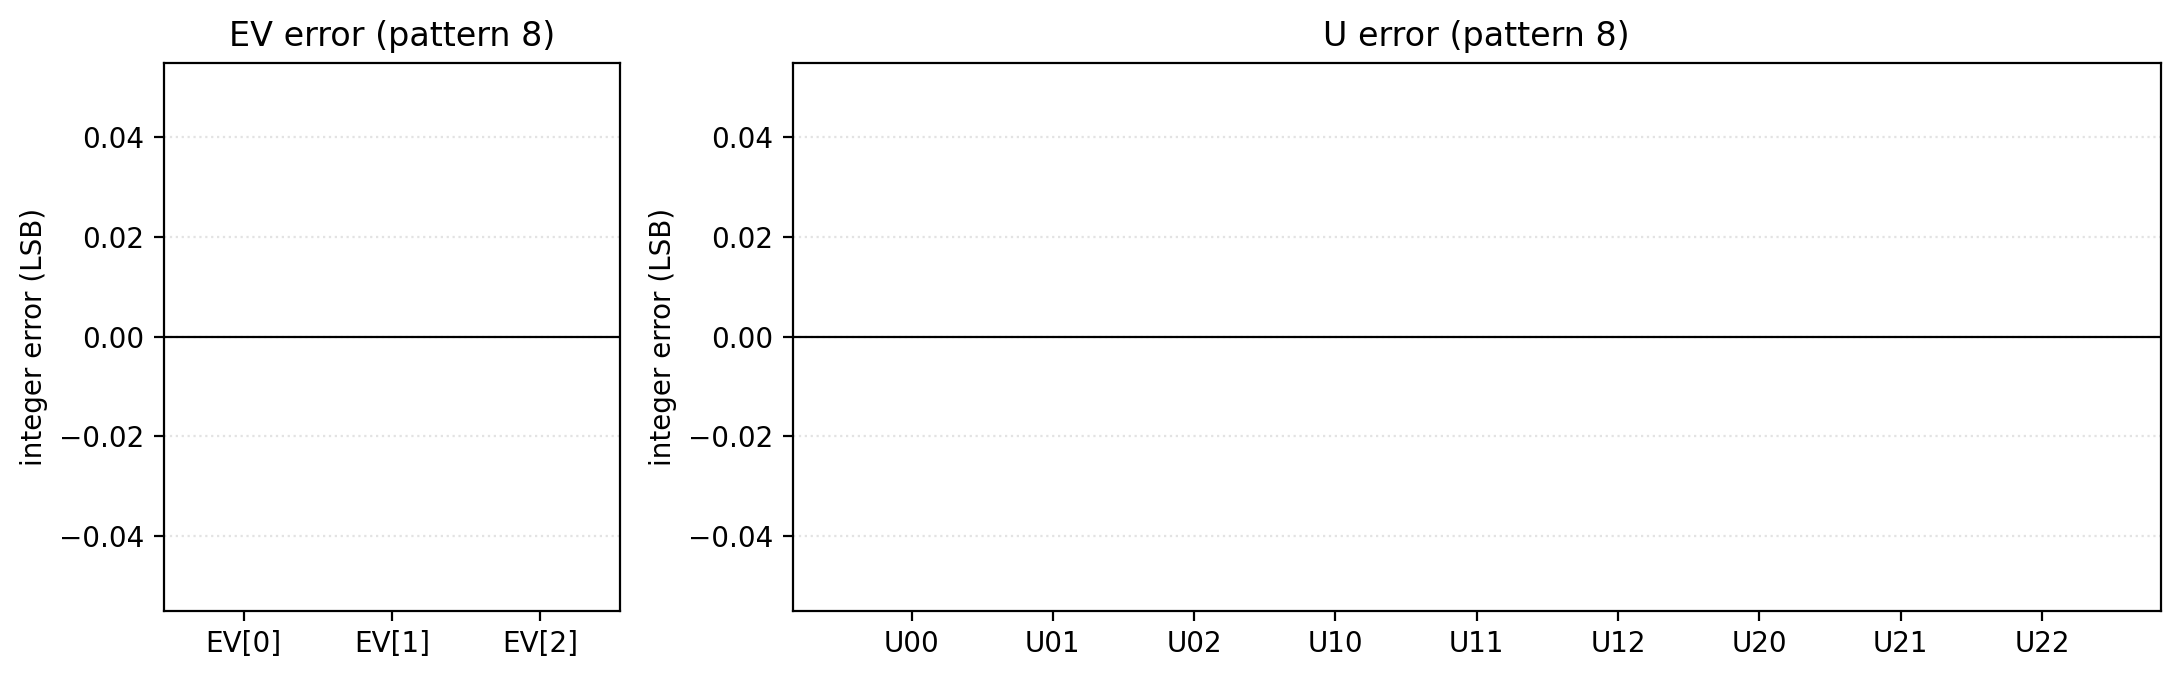
\includegraphics[width=\linewidth]{figure5.png}
    \caption{RTL vs.\ bit-true model error (pattern 8).}
    \label{fig:hw-consistency}
\end{figure}

\newpage

% ─────────────────────────────────────────────
\chapter{Section 5: Area-Time Product}

The Area-Time Product (ATP) is used to evaluate the trade-off between hardware
area and execution time. For each synthesis result, ATP is calculated as
\begin{equation}
    \mathrm{ATP}
    = \mathrm{Area} \times \mathrm{Latency} \times T_{\mathrm{clk}},
\end{equation}
where the latency is \LatencyCycles{} clock cycles and $T_{\mathrm{clk}}$ is
the clock period in nanoseconds. A lower ATP indicates a better balance
between area and timing performance.

\begin{table}[H]
\centering
\small
\caption{Area-Time Product for Different Synthesis Constraints}
\label{tab:area-time-product}
\vspace{0.15em}
\setlength{\tabcolsep}{5pt}
\renewcommand{\arraystretch}{1.0}
\begin{tabularx}{\textwidth}{c *{5}{>{\centering\arraybackslash}X}}
\toprule
\textbf{Test} &
\makecell{\textbf{Clock Period}\\\textbf{(ns)}} &
\textbf{Area} &
\makecell{\textbf{Latency}\\\textbf{(cycles)}} &
\makecell{\textbf{Execution Time}\\\textbf{(ns)}} &
\textbf{ATP} \\
\midrule
\ATPRow{1}{0.8}{6499.5}
\ATPRow{2}{0.9}{5601.9}
\ATPRow{3}{1.0}{4805.8}
\ATPRow{4}{1.1}{4759.3}
\ATPRow{5}{1.2}{4646.0}
\ATPRow{6}{1.3}{4564.3}
\ATPRow{7}{0.95}{4962.4}
\ATPRow{8}{0.975}{4892.8}
\ATPRow{9}{1.025}{4846.0}
\ATPRow{10}{0.925}{4995.9}
\ATPRow{11}{0.9225}{5016.6}
\ATPRow{12}{0.9375}{4968.0}
\ATPRow{13}{0.9625}{4923.7}
\ATPRow{14}{0.9125}{5202.9}
\ATPRow{15}{0.91875}{5133.1}
\ATPRow{16}{0.93125}{4996.5}
\ATPRow{17}{0.921875}{5000.8}
\ATPRow{19}{0.928125}{5018.7}
\ATPRow{23}{0.92225}{5013.6}
\ATPRow{24}{0.92275}{5025.1}
\ATPRow{25}{0.92325}{5013.3}
\ATPRow{26}{0.9235}{4994.0}
\ATPRow{27}{0.92375}{5003.0}
\ATPRow{28}{0.923375}{5009.5}
\ATPBestRow
\ATPRow{30}{0.923625}{5027.0}
\ATPRow{31}{0.923406}{5004.3}
\ATPRow{32}{0.923438}{4983.6}
\ATPRow{33}{0.923469}{4991.3}
\bottomrule
\end{tabularx}
\end{table}


Among the evaluated synthesis constraints, the minimum ATP is
\textbf{\num[mode=text,detect-weight=true,group-separator={,},
round-mode=places,round-precision=1]
{\ATPValue{\BestClockPeriod}{\BestArea}}}, obtained with a clock period of
\SI{\BestClockPeriod}{ns}, an area of
\num[group-separator={,},group-minimum-digits=4]{\BestArea}, and a latency of
\LatencyCycles{} clock cycles. Therefore, this configuration currently
provides the best area--timing trade-off.
% ─────────────────────────────────────────────

\newpage


\chapter{Section 6: Design Innovations}

\section{Angle-Free CORDIC via Rotational Direction Recording}

A conventional CORDIC carries an explicit angle path: each micro-rotation adds or
subtracts a stored $\arctan(2^{-i})$ constant, requiring an arctangent ROM, an angle
register, and an angle adder. In the iterative QR EVD the Givens angle is never needed
as a number, only its \emph{action} on the matrix. We therefore record only the
per-stage rotation directions in an $8$-bit \emph{rotational direction register}
(RDR) during vectoring, and replay them during rotation, reproducing the same rotation
without $\theta$.

\section{Residual-Preserving Bypass Path}

When a PE completes a vectoring operation, its $Y$ output is the eliminated
sub-diagonal entry, which is ideally zero but in fixed-point arithmetic is only a
small residual. This residual cannot simply be forced to zero, since clamping a value
that is not truly zero injects its own error. Yet if the residual is allowed to flow
into the next PE and be rotated, the rotation mixes $X$ into $Y$ through successive
shift-adds and amplifies the small residual into a much larger error. Neither
clamping nor rotating the residual is acceptable.

We resolve this with a bypass path. The downstream PE is preceded by a delay unit
that watches the upstream \texttt{OutMode}: a value produced by a vectoring operation
is tagged, and after a two-cycle alignment matching the PE latency the tag is raised
as a \texttt{Pass} flag. When \texttt{Pass} is asserted, the PE skips every
micro-rotation and the gain-scaling multiply, forwarding $X$ and $Y$ unchanged.

The residual is therefore neither clamped nor amplified: it is carried through
untouched, keeping the accumulated error bounded across iterations, while the bypassed
cycle additionally saves the rotation and scaling switching activity.

\section{Schedule-Driven Register Minimization}

Pipelining each CORDIC PE into two stages raises throughput but skews the array
outputs, so extra alignment registers are needed at the inputs and the
transpose/output buffer. Their count would dominate the area. We therefore size the
buffers from the cycle-by-cycle schedule of Fig.~\ref{fig:evd-timing} rather than by
worst-case guessing. A lifetime analysis over that schedule shows the
transpose/output buffer needs only \textbf{five} registers. The same schedule also exposes a redundant delay unit at the bottom-right diagonal,
whose value is already aligned by the adjacent two-cycle PE latency; it is replaced by
a direct wire (Fig.~\ref{fig:qrd-systolic}).

\section{Decoupled Scaling-Factor Precision}

As detailed in Section~1.4, CORDIC gain compensation is the only point that demands
extra fractional precision. Rather than widening the global fractional width $B$ and
inflating every register along the systolic datapath, we keep the datapath at $B$ and
spend the additional bits solely at the final $X\times(1/K)$ multiply-and-round, so
the precision cost is confined to a single node instead of being paid array-wide.


% ─────────────────────────────────────────────
\chapter{Section 7: Team Contributions}
% ─────────────────────────────────────────────

\begin{table}[H]
\centering
\caption{Team Contributions and Work Distribution}
\label{tab:team-work}
\vspace{0.15em}
\setlength{\tabcolsep}{8pt}
\renewcommand{\arraystretch}{1.2}
\begin{tabularx}{\textwidth}{>{\raggedright\arraybackslash}Xcc}
\toprule
\textbf{Work Item} &
\makecell{\textbf{MING-HONG,LIN}} &
\makecell{\textbf{YING-CHENG,CHEN}} \\
\midrule
Algorithm Research and Configuration Analysis        & \ding{51} & \ding{51} \\
Fixed-Point Bit-True Model Development               & \ding{51} & \ding{51} \\
Total Word-Length and Accuracy Analysis              & \ding{51} & \ding{51} \\
Hardware Architecture and Control Flow Design        & \ding{51} & \ding{51} \\
RTL Design                                           & \ding{51} & \ding{51} \\
Testbench Development and Unit Verification          & \ding{51} & \ding{51} \\
Behavioral Simulation                                & \ding{51} & \ding{51} \\
Logic Synthesis and Area/Timing Analysis              & \ding{51} & \ding{51} \\
Post-Synthesis Simulation                            & \ding{51} & \ding{51} \\
Hardware Optimization                                & \ding{51} & \ding{51} \\
Area-Time Product Evaluation                         & \ding{51} & \ding{51} \\
Result Analysis and Visualization                    & \ding{51} & \ding{51} \\
Report Writing                                       & \ding{51} & \ding{51} \\
\midrule
\textbf{Weight}                                      & \textbf{50\%} & \textbf{50\%} \\
\bottomrule
\end{tabularx}
\end{table}

\end{document}


